% Assignment 4 report -- compile with LuaLaTeX (needed for Devanagari shaping):
%   lualatex report.tex   (run twice for references)
\documentclass[10pt,a4paper]{article}
\usepackage[margin=2cm]{geometry}
\usepackage{fontspec}
\usepackage{amsmath,amssymb}
\usepackage{graphicx}
\usepackage{booktabs}
\usepackage{tabularx}
\usepackage{array}
\usepackage{float}
\usepackage{caption}
\usepackage[shortlabels]{enumitem}
\usepackage{xcolor}
\usepackage{microtype}
\usepackage[colorlinks=true,linkcolor=blue!50!black,urlcolor=blue!50!black,citecolor=blue!50!black]{hyperref}

% Devanagari font: Nirmala UI (Windows) or Noto Sans Devanagari (Overleaf / Linux).
\IfFontExistsTF{Nirmala UI}
  {\newfontfamily\hindifont{Nirmala UI}[Script=Devanagari,Renderer=HarfBuzz]}
  {\newfontfamily\hindifont{Noto Sans Devanagari}[Script=Devanagari,Renderer=HarfBuzz]}
\newcommand{\hi}[1]{{\hindifont #1}}

\graphicspath{{../figures/}}
\setlist{itemsep=1pt,topsep=3pt}
\setlength{\emergencystretch}{3em}
\captionsetup{font=small,labelfont=bf}
\newcolumntype{Y}{>{\raggedright\arraybackslash}X}
\newcommand{\code}[1]{\texttt{#1}}

\title{\textbf{Assignment 4: Machine Translation with LSTM, GRU\\and Encoder--Decoder Models}\\[2pt]
\large CS4101 $|$ CS6103 --- English $\rightarrow$ Hindi on the IIT Bombay corpus}
\author{Anshul Kaushal (2611AI10) \and Aditya Sharma (2611CS11) \and Roland Zohmingthana (2611MC03)}
\date{November 2026}

\begin{document}
\maketitle

\begin{abstract}
\noindent We implement vanilla RNN, LSTM and GRU cells from basic tensor operations, verify them
against PyTorch to $\le 4\times10^{-15}$ (values, final states and gradients, on padded batches), and
build a configurable encoder--decoder translator (no attention) trained with teacher forcing and decoded
greedily. On a fixed-seed subset of 20{,}000 IIT Bombay English--Hindi pairs of 1--10 tokens, four
configurations (LSTM/GRU $\times$ $H\in\{64,128\}$) are trained for 10 epochs. GRU-128 is selected by
validation BLEU-4 (2.56) and reaches \textbf{2.20 BLEU-4} on the test set (loss 3.368, perplexity 29.0,
token accuracy 48.5\%). Our own corpus BLEU-4 equals sacrebleu exactly on every evaluation. Absolute
BLEU is low because the short end of the corpus is dominated by glossary entries and UI strings and
26.6\% of Hindi test tokens are outside the training vocabulary; we analyse these limits, the gradient flow
of the three cells, exposure bias, SVO$\to$SOV reordering through a fixed-size state, and the stability of
the model ranking across seeds.
\end{abstract}

\section{Dataset and tokenisation}

\paragraph{Source and cleaning.} The official \emph{train} split of \code{cfilt/iitb-english-hindi}
(1{,}659{,}083 pairs, only 1{,}093{,}624 distinct English sentences) is downloaded as a parquet file with
\code{urllib} (no Hugging Face libraries). The official dev/test splits are news sentences that are
nearly all longer than 10 tokens, so all three of our splits are drawn from the train split. A pair is
kept if the English side contains only ASCII letters, digits and common punctuation (this removes
software strings with \code{\%s}, \code{\_}, \code{\&}, markup and mis-encoded text), the Hindi side only
Devanagari, digits and punctuation with at least one Devanagari letter (removes untranslated English and
mojibake, i.e.\ UTF-8 Hindi mis-decoded as Latin-1), both sides have 1--10 tokens, and neither side is more than $3\times+2$ longer
than the other (Table~\ref{tab:funnel}).

\paragraph{Fixed-seed subset.} The 667{,}057 clean pairs are permuted with
\code{numpy.random.default\_rng(42)}; walking through the permutation we keep only the first occurrence of
each English sentence (one randomly chosen translation per duplicated source; this also guarantees that
no source sentence occurs in two splits) and stop at 20{,}000 pairs, split 16{,}000 / 2{,}000 / 2{,}000
(train/validation/test).

\begin{table}[H]
\centering\small
\begin{tabular}{lr}
\toprule
Filter step & pairs \\
\midrule
invalid English characters & 126{,}947 \\
invalid Hindi characters & 92{,}625 \\
outside 1--10 tokens & 769{,}421 \\
length ratio & 3{,}033 \\
\textbf{kept} (319{,}291 distinct English) & \textbf{667{,}057} \\
\bottomrule
\end{tabular}
\caption{Cleaning funnel on the 1{,}659{,}083 raw training pairs.}
\label{tab:funnel}
\end{table}

\paragraph{Tokenisation.} English: NFKC, lower-casing, curly$\to$straight quotes and a regular expression
that keeps words (with clitics such as \code{'s}), numbers and single punctuation marks. Hindi needs a
Devanagari-aware rule: vowel signs (\hi{ि}, \hi{ा}), \emph{virama} \hi{्}, \emph{anusvara} \hi{ं} and
\emph{nukta} \hi{़} are combining marks that Python's \verb|\w| does not match, so a \verb|\w+| tokeniser
would split \hi{हिन्दी} into fragments. We (i) apply Unicode NFC and remove zero-width joiners so each word
has one code-point sequence; (ii) handle \textbf{sentence-ending punctuation}: the corpus ends Hindi
sentences with the \emph{danda} \hi{।}, an ASCII ``.'' or a pipe ``|'' inconsistently; a sentence-final
``.''/``|'' is mapped to \hi{।} and \hi{।}/\hi{॥} are always split off as separate tokens. Otherwise
\hi{है।}, \hi{है.} and \hi{है} would be three vocabulary items, inflating the vocabulary and UNK rate, and
BLEU would penalise a correct final verb because of an arbitrary punctuation choice; (iii) every other
punctuation mark is a separate token and maximal runs of Devanagari letters/signs form words. The same
tokeniser produces the training targets, the references and the hypotheses; BLEU is computed on these
pre-tokenised strings (\code{tokenize="none"} in sacrebleu).

\paragraph{Vocabulary and statistics.} Vocabularies are built on the training split with
\code{min\_freq}~$=2$ (singletons become \code{<unk>}, which also teaches the model to handle unseen words)
plus four specials: \textbf{English 4{,}899} and \textbf{Hindi 4{,}974} entries. Table~\ref{tab:data} gives
the split sizes and unknown-token rates. Mean length is only $\approx3.7$ tokens: 47\% of test sources have
1--2 tokens, because the short end of IITB consists largely of dictionary/glossary entries
(\emph{pistachio nut}~$\to$~\hi{पिस्ता}) and UI strings (\emph{failed to create user}). Hindi has more
types and a higher UNK rate than English: it inflects nouns, adjectives and verbs for gender, number and
case (\hi{गया/गई/गए}) and spells loanwords in several ways (\hi{फ़ाइल/फाइल}, \hi{पहुंच/पहुँच}). 70\% of
Hindi training types (11{,}357 of 16{,}327) occur only once.

\begin{table}[H]
\centering\small
\begin{tabular}{llrrrrr}
\toprule
split & language & sentences & tokens & types & \code{<unk>} tokens & UNK rate \\
\midrule
train & English & 16{,}000 & 57{,}478 & 14{,}303 & 9{,}408 & 16.37\% \\
train & Hindi   & 16{,}000 & 58{,}556 & 16{,}327 & 11{,}357 & 19.40\% \\
val   & English & 2{,}000 & 7{,}367 & 3{,}331 & 1{,}757 & 23.85\% \\
val   & Hindi   & 2{,}000 & 7{,}593 & 3{,}604 & 1{,}975 & 26.01\% \\
test  & English & 2{,}000 & 7{,}521 & 3{,}374 & 1{,}735 & 23.07\% \\
test  & Hindi   & 2{,}000 & 7{,}690 & 3{,}704 & 2{,}042 & 26.55\% \\
\bottomrule
\end{tabular}
\caption{Split sizes and token-level unknown rates (vocabulary from train, \code{min\_freq}=2; the train
rate is the share of singleton tokens).}
\label{tab:data}
\end{table}

\section{Task 1: recurrent cells and encoder--decoder}

\subsection{Cells, initialisation and padding}
All cells use only matrix products, additions, element-wise products, \code{sigmoid} and \code{tanh},
with PyTorch's weight layout ($W_{ih}\in\mathbb R^{GH\times d}$, $W_{hh}\in\mathbb R^{GH\times H}$, two
biases; gate order $i,f,g,o$ for the LSTM and $r,z,n$ for the GRU):
\begin{align*}
\text{RNN:}\;& h_t=\tanh(W_{ih}x_t+b_{ih}+W_{hh}h_{t-1}+b_{hh})\\
\text{LSTM:}\;& [i,f,g,o]=W_{ih}x_t+b_{ih}+W_{hh}h_{t-1}+b_{hh},\quad
c_t=\sigma(f)\odot c_{t-1}+\sigma(i)\odot\tanh(g),\quad h_t=\sigma(o)\odot\tanh(c_t)\\
\text{GRU:}\;& r=\sigma(W_{ir}x_t+b_{ir}+W_{hr}h_{t-1}+b_{hr}),\;
z=\sigma(W_{iz}x_t+b_{iz}+W_{hz}h_{t-1}+b_{hz}),\\
&n=\tanh\big(W_{in}x_t+b_{in}+r\odot(W_{hn}h_{t-1}+b_{hn})\big),\quad h_t=(1-z)\odot n+z\odot h_{t-1}.
\end{align*}
\textbf{Initialisation:} every weight and bias is drawn i.i.d.\ from $\mathcal U(-1/\sqrt H,1/\sqrt H)$
using the global torch generator, which is seeded immediately before each model is built. This keeps gate
pre-activations at unit order so sigmoids/tanh start unsaturated. We deliberately do not add a
forget-gate bias of $+1$, so that all three cells start from the same distribution in the gradient
experiment. Embeddings use PyTorch's $\mathcal N(0,1)$ default (padding row zero) and the output layer
its default uniform initialisation.

\textbf{Padded batches:} a \code{RecurrentLayer} runs a cell over time given the true lengths $L_b$. For
$t\ge L_b$ the state of sequence $b$ is frozen with \code{torch.where} and its output is zero, so the
returned final state is the state after the last real token (the semantics of
\code{pack\_padded\_sequence}) and padding affects neither the state nor the gradients.

\subsection{Verification against PyTorch}
We copy our weights into \code{nn.\{RNN,LSTM,GRU\}Cell} and \code{nn.\{RNN,LSTM,GRU\}}, and compare in
float64 on a padded batch with lengths $(7,5,3,1,6)$ fed to the built-in layer through
\code{pack\_padded\_sequence}. This is the only use of built-in recurrent layers. Table~\ref{tab:verify}:
all differences are at machine precision and padded outputs are exactly zero.

\begin{table}[H]
\centering\small
\begin{tabular}{lcccccc}
\toprule
cell & single step & outputs & final state(s) & padded out $=0$ & $\nabla$ input & $\nabla$ weights \\
\midrule
RNN  & 1.1e-16 & 1.1e-16 & 1.1e-16 & yes & 2.2e-16 & 3.6e-15 \\
LSTM & 2.2e-16 & 5.6e-17 & 1.1e-16 & yes & 1.1e-16 & 5.6e-16 \\
GRU  & 1.1e-16 & 1.9e-16 & 1.7e-16 & yes & 2.2e-16 & 1.8e-15 \\
\bottomrule
\end{tabular}
\caption{Maximum absolute difference between our cells and PyTorch (float64).}
\label{tab:verify}
\end{table}

\subsection{Parameter count for $d=128$, $H=256$}
A cell with $G$ gate blocks has $G(dH+H^2+2H)$ parameters: \textbf{RNN 98{,}816}, \textbf{GRU 296{,}448}
($G=3$), \textbf{LSTM 395{,}264} ($G=4$); the counted \code{numel} agrees. The ratio LSTM/GRU is exactly
$4/3$ for every $d,H$: each gate block (input matrix, recurrent matrix, two biases) has the same size in
both cells, and the LSTM has four blocks (input, forget, output gate, cell candidate) while the GRU has three
(reset, update, candidate). The GRU couples ``forget'' and ``input'' into one update gate ($z$ and $1-z$) and
has no separate cell state, hence no output gate. The second bias is required in the GRU because $b_{hn}$
sits inside the reset product; for the LSTM it is redundant but kept for PyTorch compatibility.

\subsection{Gradient flow}
For $T\in\{10,25,50,100\}$, $B=16$, $d=32$, $H=64$ and $x\sim\mathcal N(0,I)$ we compute
$\|\partial\|h_T\|_2^2/\partial x_1\|_2$ per sequence, average over the batch and over seeds 0--4. For seed $s$
the cell is initialised after \code{torch.manual\_seed(s)} and the inputs come from a separate generator
seeded with $s$, so all cells see identical inputs. We use float64 on CPU to avoid underflow
(Figure~\ref{fig:grad}, Table~\ref{tab:grad}).

\begin{figure}[H]
\centering
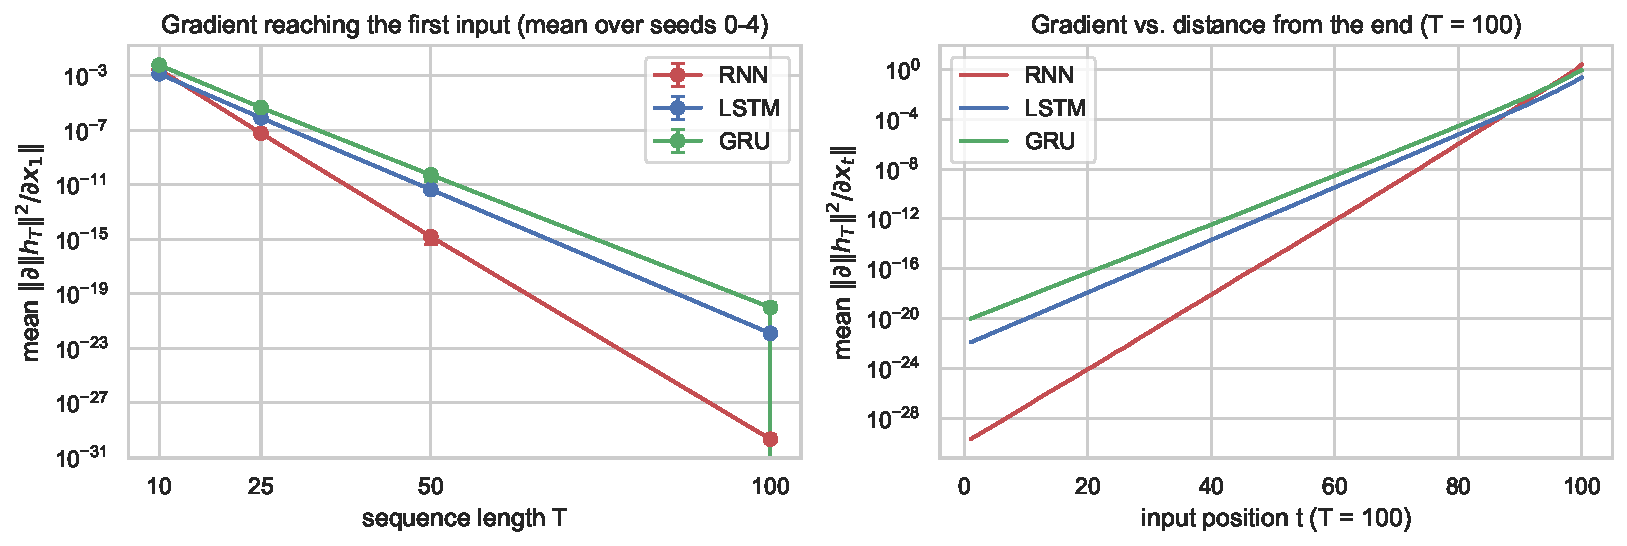
\includegraphics[width=\textwidth]{gradient_flow.pdf}
\caption{Left: mean gradient norm reaching $x_1$ versus $T$ (log scale, error bars = std over seeds).
Right: gradient norm with respect to every $x_t$ for $T=100$.}
\label{fig:grad}
\end{figure}

\begin{table}[H]
\centering\small
\begin{tabular}{rccc}
\toprule
$T$ & RNN & LSTM & GRU \\
\midrule
10  & $2.80\times10^{-3}$ & $1.36\times10^{-3}$ & $5.98\times10^{-3}$ \\
25  & $5.85\times10^{-8}$ & $7.94\times10^{-7}$ & $4.50\times10^{-6}$ \\
50  & $1.53\times10^{-15}$ & $4.33\times10^{-12}$ & $5.17\times10^{-11}$ \\
100 & $2.07\times10^{-30}$ & $1.22\times10^{-22}$ & $9.65\times10^{-21}$ \\
\midrule
avg.\ per-step factor & 0.50 & 0.61 & 0.63 \\
\bottomrule
\end{tabular}
\caption{Mean $\|\partial\|h_T\|^2/\partial x_1\|$ over seeds 0--4; last row: $e^{-\text{slope}}$ of the
$T=100$ log-profile.}
\label{tab:grad}
\end{table}

\paragraph{Observation.} All curves are straight lines on the log scale: the gradient reaching $x_1$
\emph{vanishes exponentially} in $T$, since it is a product of $T-1$ Jacobians
$\partial h_t/\partial h_{t-1}$. For the \textbf{RNN} each Jacobian is $\mathrm{diag}(1-h_t^2)W_{hh}$; with
$\mathcal U(\pm1/\sqrt H)$ the spectral radius of $W_{hh}$ is $\approx1/\sqrt3\approx0.58$ and $\tanh'\le1$,
so each step halves the gradient (factor 0.50), leaving $10^{-30}$ after 100 steps. The \textbf{LSTM} starts
\emph{below} the RNN at $T=10$, because the output gate and the extra $\tanh(c_t)$ each scale $h_T$ by about
$0.5$, but it decays more slowly and is eight orders of magnitude larger at $T=100$. Its cell state has an
additive path $c_t=f_t\odot c_{t-1}+\dots$ whose Jacobian is just $\mathrm{diag}(f_t)$, with no weight matrix
and no squashing. The \textbf{GRU} is largest at every $T$: $h_t=z\odot h_{t-1}+(1-z)\odot n$ is a gated
identity path, and there is no output gate. At initialisation all gates are $\approx\sigma(0)=0.5$, so gated
cells \emph{also} vanish; gating is no guarantee. The difference is that their per-step factor is a learnable,
input-dependent gate that training can drive towards 1 (a forget bias of $+1$ alone gives $\sigma(1)=0.73$),
whereas the RNN's factor is fixed by $W_{hh}$ and tanh saturation.

\subsection{Encoder--decoder model}
The \textbf{encoder} is an embedding followed by \code{num\_layers} of our recurrent layers (LSTM or GRU),
run over the true source lengths (source $+$ \code{<eos>}). Its final state ($h$, and $c$ for the LSTM) is the
only information passed on: a fixed-size summary with no attention. The \textbf{decoder} is an embedding
followed by the same cell type initialised with that state, then dropout and a linear layer to the Hindi
vocabulary. Configurable options: cell type, embedding size, hidden size, number of layers, dropout. During
\textbf{training (teacher forcing)} the decoder input at step $t$ is the \emph{reference} token $y_{t-1}$
(\code{<bos>} at $t=1$), and the loss is the token cross-entropy over all non-pad targets including
\code{<eos>}. For \textbf{inference (greedy)} we start from \code{<bos>}, feed back the arg-max token, and stop when
all sentences have emitted \code{<eos>} or after 20 steps.

\subsection{Teacher forcing versus free-running decoding}
Under teacher forcing the decoder is always conditioned on the true prefix $y_{<t}$; in free running it is
conditioned on its own predictions $\hat y_{<t}$. During training it never sees its own mistakes
(\emph{exposure bias}), so an early error moves it into a state distribution it was never trained on, and the
errors compound. \textbf{Example} (final model, validation): \emph{``failed to create user''}, reference
\hi{उपयोक्ता बनाने में विफल}. With teacher forcing the arg-max predictions are
\hi{उपयोक्ता चुनें में विफल} \code{<eos>}: the second word is wrong (\hi{चुनें} ``select'' instead of
\hi{बनाने} ``create''), but because step~3 is fed the reference \hi{बनाने}, the model still predicts the
correct \hi{में विफल}. In free running \hi{चुनें} is fed back. It is the imperative that ends thousands of
UI strings, so the decoder emits \code{<eos>} at once and outputs \hi{उपयोक्ता चुनें} (``select user''):
fluent, but ``failed'' is lost. Figure~\ref{fig:exposure} quantifies this. Both regimes agree at position 1
(same input), but from position 2 free-running accuracy drops well below teacher-forced accuracy
(e.g.\ 0.20 vs 0.36 at position 5). Teacher-forced accuracy rises again at late positions because long
references end in the predictable \hi{है ।}~\code{<eos>}.

\begin{figure}[H]
\centering
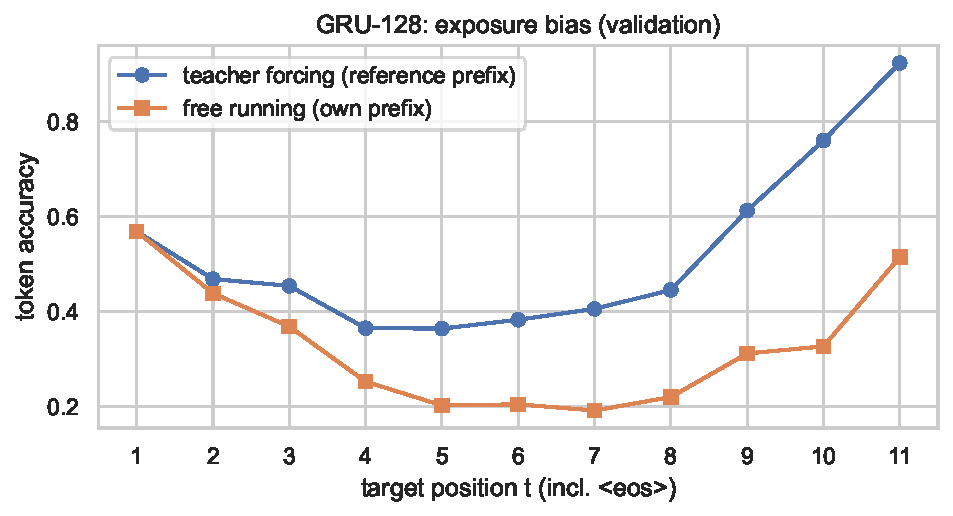
\includegraphics[width=0.55\textwidth]{exposure_bias.pdf}
\caption{Position-wise token accuracy on the validation set for GRU-128 under teacher forcing and in free
running.}
\label{fig:exposure}
\end{figure}

\subsection{Training, metrics and BLEU}
Per epoch we log the training loss, perplexity ($e^{\text{loss}}$) and token accuracy (arg-max $=$
reference over non-pad positions, teacher-forced, accumulated with dropout active); the same three on
validation; and validation BLEU-4 of greedy translations against the original tokenised references.
Reference OOV words are not replaced by \code{<unk>}, so an output \code{<unk>} never matches.

\paragraph{Own BLEU-4.} Corpus-level $\mathrm{BLEU}=\mathrm{BP}\cdot\exp(\frac14\sum_{n=1}^4\log p_n)$ with
clipped $n$-gram counts summed over the whole corpus before dividing,
$p_n=\sum_s\sum_g\min(c_h(g),c_r(g))/\sum_s\max(|h_s|-n+1,0)$, and $\mathrm{BP}=\min(1,e^{1-r/c})$ for total
reference length $r$ and hypothesis length $c$. Optional NIST ``exp'' smoothing (sacrebleu's default) replaces
the $k$-th zero precision by $1/(2^k\,\mathrm{total}_n)$. \textbf{Comparison with sacrebleu} on the same
pre-tokenised strings (\code{tokenize="none"}): the maximum difference over 400 random test corpora (both
smoothing modes) is $1.4\times10^{-14}$, and the two scores agree to within $9\times10^{-16}$ in all 40 per-epoch validation
evaluations and on the test set. sacrebleu is used for all model selection. With sacrebleu's default
\code{13a} tokeniser instead, test BLEU would be 1.07 rather than 2.20, because \code{13a} re-tokenises our
strings (e.g.\ splitting \code{<unk>} into three tokens). This is why both scores must be computed on the same
pre-tokenised text.

\paragraph{Why BLEU under-rewards valid Hindi.} Hindi marks grammatical roles with postpositions
(\hi{ने}, \hi{को}, \hi{से}, \hi{में}) rather than position, so constituent order is relatively free. BLEU
counts surface $n$-gram overlap with a single reference, so a meaning-preserving reordering loses most 3- and
4-grams. In our constructed example (reference \hi{राम ने सीता को किताब दी ।}) the reordering
\hi{सीता को राम ने किताब दी ।} (same meaning) scores \textbf{35.9}, the synonym \hi{पुस्तक} for \hi{किताब}
scores 48.9, and the sentence with the \emph{opposite} meaning \hi{सीता ने राम को किताब दी ।} (Sita gave
Ram) scores \textbf{47.3}, higher than the correct reordering. Spelling variants (\hi{गई/गयी},
\hi{फ़ाइल/फाइल}), optional honorific plurals and the choice between Sanskritised and English loanwords
(\hi{संगणक/कंप्यूटर}) are penalised in the same way, and inflection multiplies the forms that must match
exactly.

\section{Task 2: cell type and hidden size}

\paragraph{Fixed hyperparameters (all four runs).} Embedding size 128, one layer, dropout 0.3 (on
embeddings and before the output layer), Adam with lr $3\times10^{-3}$ and $\beta=(0.9,0.999)$, batch size
64, gradient-norm clipping 1.0, 10 epochs, greedy decoding of at most 20 steps, \code{min\_freq}~2, seed 42
for initialisation and shuffling (so all runs see the same batch order). The learning rate and batch size were
chosen in a short pilot on the validation set (LSTM-128 with lr $10^{-3}$ was still improving at epoch 10;
lr $3\times10^{-3}$ converged within the budget; batch 32 was only marginally better at twice the cost).
The checkpoint of each run is its earliest epoch with maximum validation sacreBLEU.

\begin{table}[H]
\centering\footnotesize
\setlength{\tabcolsep}{4pt}
\begin{tabular}{lrrcccccccc}
\toprule
model & params & time (s) & ckpt ep. & val BLEU & val loss & val ppl & val acc & train loss & train acc & min val-loss ep. \\
\midrule
LSTM-64  & 1{,}686{,}382 & 124.1 & 9  & 1.51 & 3.718 & 41.18 & 0.443 & 3.719 & 0.414 & 10 \\
GRU-64   & 1{,}661{,}550 & 130.1 & 8  & 1.50 & 3.603 & 36.72 & 0.452 & 3.621 & 0.420 & 10 \\
LSTM-128 & 2{,}169{,}582 & 129.7 & 8  & 1.65 & 3.621 & 37.39 & 0.461 & 3.325 & 0.440 & 10 \\
GRU-128  & 2{,}103{,}534 & 129.8 & 10 & \textbf{2.56} & \textbf{3.446} & \textbf{31.37} & \textbf{0.473} & 2.634 & 0.491 & 8 \\
\bottomrule
\end{tabular}
\caption{Task 2 runs. Time = total training time over 10 epochs (excluding validation decoding); metrics at
the checkpoint epoch. Our BLEU equals sacrebleu in every row.}
\label{tab:runs}
\end{table}

\begin{figure}[H]
\centering
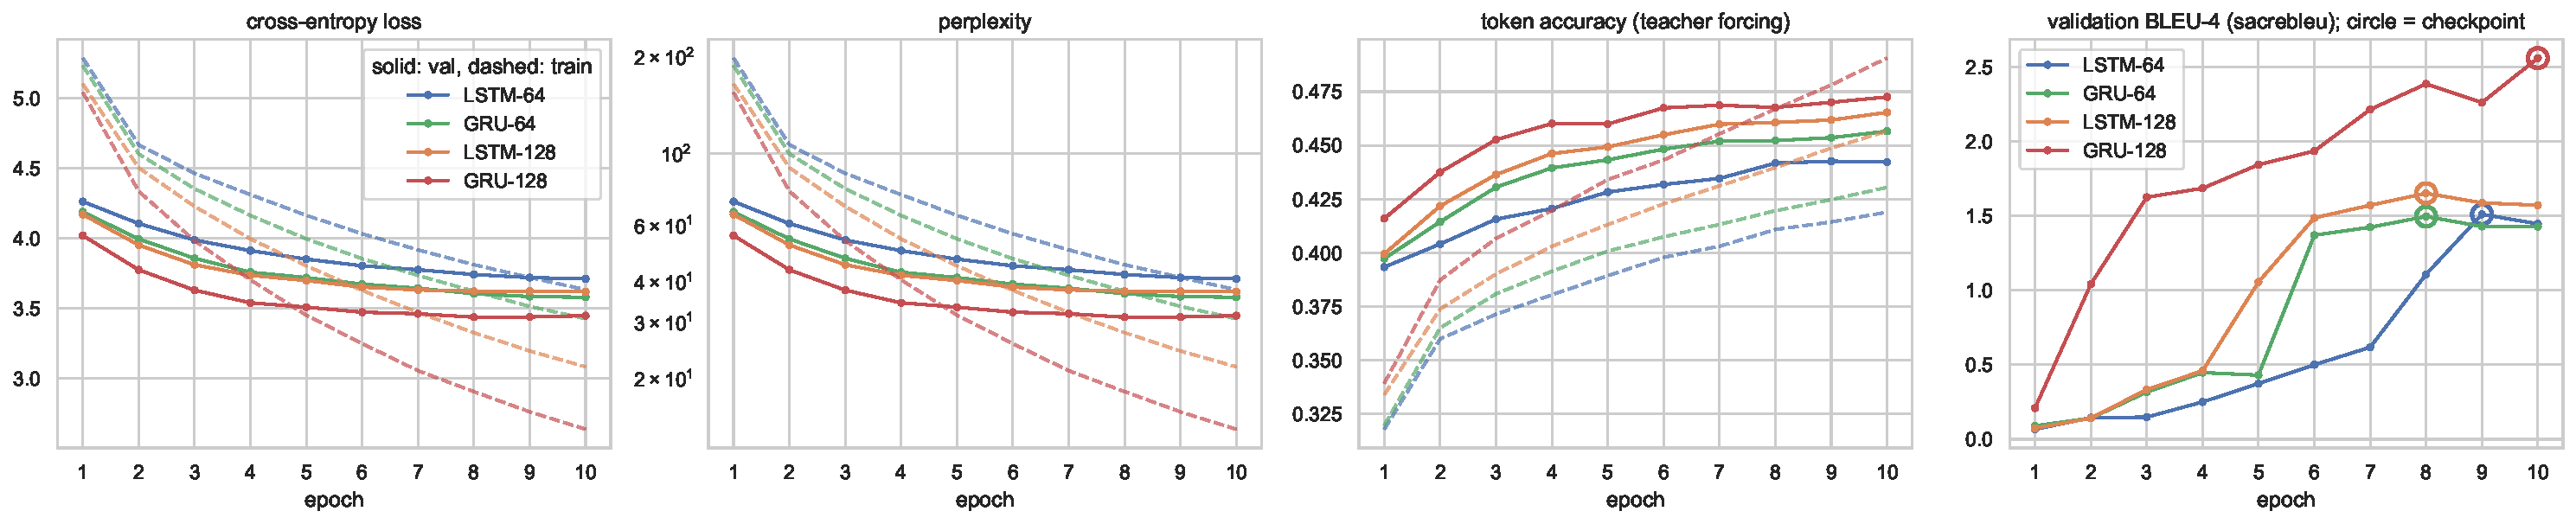
\includegraphics[width=\textwidth]{training_curves.pdf}
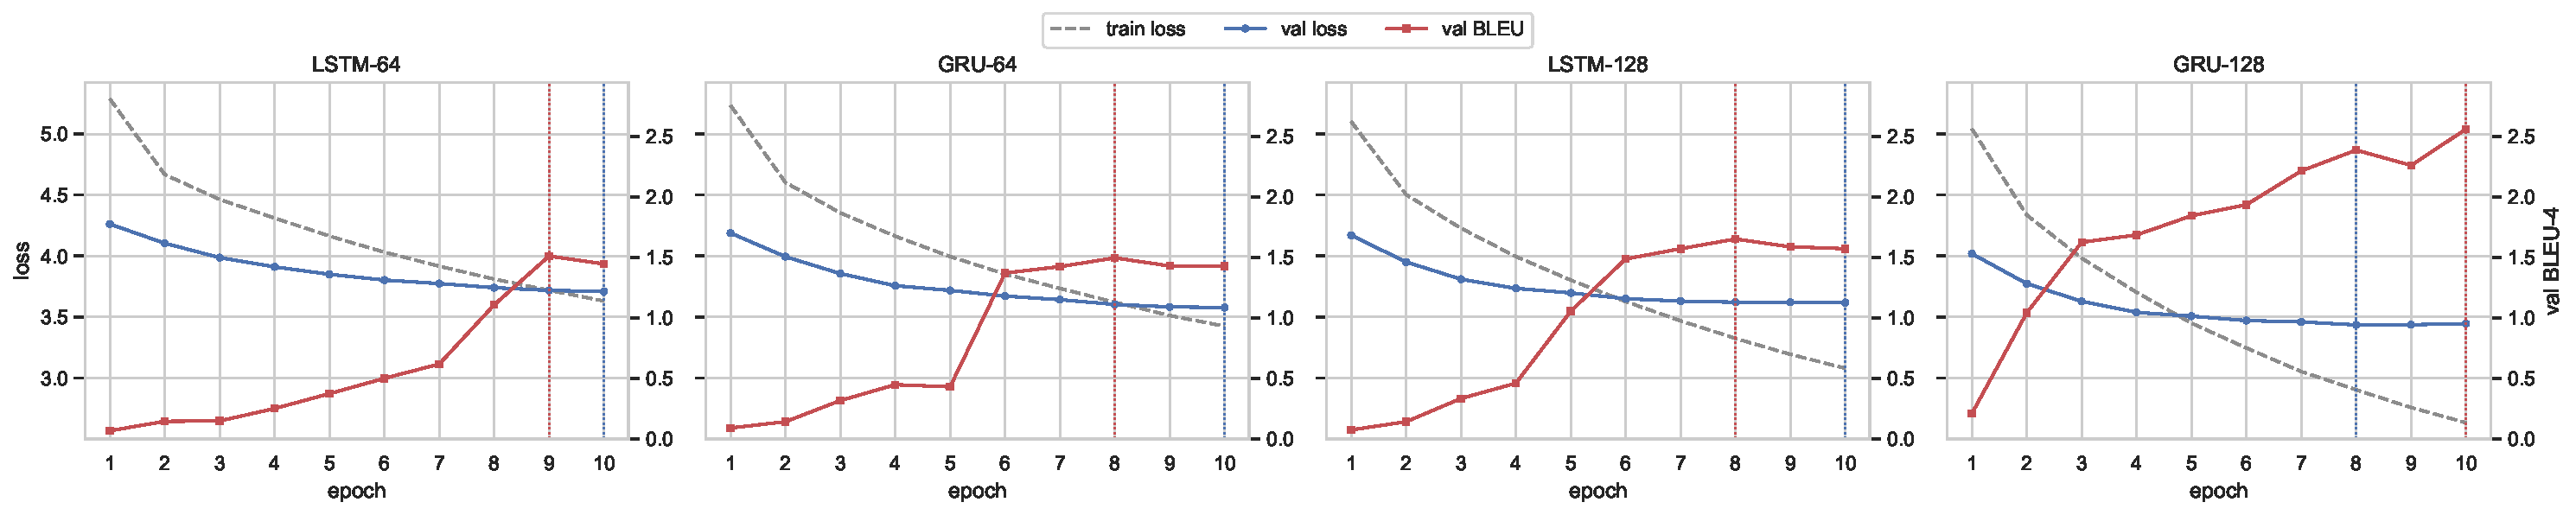
\includegraphics[width=\textwidth]{loss_vs_bleu.pdf}
\caption{Top: training (dashed) and validation (solid) loss, perplexity and token accuracy, and validation
BLEU-4 (circle = checkpoint) for all runs. Bottom: per-run loss against validation BLEU; dotted lines mark the
minimum validation loss (blue) and the maximum BLEU (red).}
\label{fig:curves}
\end{figure}

\paragraph{Effect of cell type and hidden size.}
\emph{Quality:} GRU-128 is clearly best (BLEU 2.56, perplexity 31.4). The other three lie within
0.15 BLEU of each other. A larger $H$ helps both cells (lower validation loss), and the GRU gains more. With
$\le 11$ time steps there are no long-range dependencies for the LSTM's separate memory to exploit, and the
GRU, with fewer parameters per unit and the strongest gradient path (Table~\ref{tab:grad}), learns faster in
10 epochs: its validation BLEU jumps already at epoch 2--3.
\emph{Cost:} the recurrent cells are a small part of each model. For GRU-128, the two embedding tables
(627{,}072 $+$ 636{,}672) and the output layer (641{,}646) hold 1.91\,M of 2.10\,M parameters, and the
encoder and decoder GRUs only 99{,}072 each. This is a direct consequence of the 4.9k/5.0k vocabularies:
doubling $H$ adds only $0.44$--$0.48$\,M parameters, and LSTM vs GRU differs by $\le66$k. Training
time is 130--138\,s for every run because, with $T\le11$ and small matrices, the GPU is limited by the Python
time loop and kernel launches, not by FLOPs (wall-clock times vary by several seconds between executions, so the small differences between runs are not meaningful).
\emph{Under/over-fitting:} with dropout active, LSTM-64 still has training loss $\approx$ validation loss
(3.63 vs 3.71 at epoch 10), and both are still decreasing, so it is capacity- and epoch-limited
(\textbf{under-fitting}). GRU-128 reaches training loss 2.63 against validation 3.45, and its validation loss
bottoms out at epoch 8 and then rises (the \textbf{onset of over-fitting}). The vocabulary statistics explain
why this happens so early: 70\% of Hindi training types are singletons and 26\% of held-out Hindi tokens are
unknown, so extra capacity is spent memorising rare training words that never recur, and a quarter of all
reference tokens cannot be produced by any model with this vocabulary (\code{<unk>} never matches). The
models therefore learn frequent function words, postpositions and sentence frames well, but not content
words.

\paragraph{Validation BLEU or validation loss as checkpoint criterion?} Across epochs the two are strongly
anti-correlated (Spearman $-0.94$ to $-0.99$), yet they pick different epochs: for GRU-128 the loss picks
epoch 8 and BLEU picks epoch 10 (2.39$\to$2.56 although the loss rises slightly), and for LSTM-64/128
BLEU peaks at epoch 9/8 while the loss is still falling. We consider validation BLEU the better criterion for
this task, for three reasons. (i) It evaluates free-running greedy output, which is what is deployed, whereas
the loss is teacher-forced and blind to exposure bias. (ii) Loss and token accuracy reward predicting
\code{<unk>} for the 26\% OOV reference tokens, which BLEU correctly never rewards; a model that becomes more
confident about \code{<unk>} improves its loss without translating better. (iii) It matches the selection and
reporting metric. Its drawback, visible in Figure~\ref{fig:curves}, is \emph{noise}. At BLEU $\approx2$ the
epoch-to-epoch wiggles (GRU-128: 2.39, 2.26, 2.56; LSTM-64: 1.51, 1.45) are as large as genuine differences,
so the smoother validation loss is the more reliable \emph{over-fitting} signal. A combined rule, maximising
BLEU among epochs whose loss is within a tolerance of its minimum, would be a sensible compromise.

\section{Task 3: final model}

\paragraph{Selection and justification.} Ranking by checkpoint validation sacreBLEU gives GRU-128 (2.56)
$>$ LSTM-128 (1.65) $>$ LSTM-64 (1.51) $>$ GRU-64 (1.50); no tie-break is needed. GRU-128 also has the lowest
validation loss and perplexity and the highest token accuracy, so all validation metrics agree. It has
fewer parameters than LSTM-128, trains no slower than the others, and is ranked first under every seed tested
(below). Its checkpoint is epoch 10.

\paragraph{Test set (evaluated once).} \textbf{BLEU-4 2.20} (own) $=$ \textbf{2.20} (sacrebleu,
\code{tokenize="none"}), loss 3.368, perplexity 29.02, token accuracy 48.45\%. The test BLEU is a little below
the validation BLEU used for selection (2.56), as expected after choosing the maximum of 40 noisy validation
measurements.

\begin{table}[H]
\centering\small
\begin{tabularx}{\textwidth}{rYYY}
\toprule
\# & English source & Hindi reference & GRU-128 output \\
\midrule
1 & web development & \hi{वेब विकास} & \hi{वेब विकास} \\
2 & a tuberculosis of a spine & \hi{रीढ़ का तपेदिक ।} & \code{<unk>} \hi{का} \code{<unk>} \\
3 & grand turk & \hi{क़िबलाआलम} & \code{<unk> <unk>} \\
4 & steganalysis software & \hi{स्टेगएनालिसिस सॉफ़्टवेयर} & \code{<unk> <unk>} \\
5 & dagger & \hi{डैगर} & \code{<unk>} \\
6 & plotting head is related to graphics . & \hi{आलेखन शीर्ष , ग्राफिक्स से संबंधित होता है ।} & \code{<unk> <unk>} \hi{के लिए} \code{<unk> <unk>} \hi{।} \\
7 & insert advanced send options & \hi{उन्नत प्रेषण विकल्प डालें} & \hi{नया डाक को} \code{<unk>} \hi{करें} \\
8 & and i 'll show you in a problem . & \hi{मैं आपको सवाल में दिखता हूँ} & \hi{और मैंने तुमको उससे} \code{<unk> <unk>} \hi{है ?} \\
9 & adhesive tape & \hi{आसंजक टेप} & \code{<unk>} \\
10 & acta sociologica & \hi{एक्टा सोशियोलॉजिका} & \code{<unk> <unk>} \\
\bottomrule
\end{tabularx}
\caption{The first 10 test translations.}
\label{tab:first10}
\end{table}

\paragraph{Error analysis.} Table~\ref{tab:errors} classifies erroneous test translations by error type.
Unknown words dominate: most outputs contain \code{<unk>}, and transliterated names and numbers cannot be
copied without an attention or copy mechanism.

\begin{table}[H]
\centering\small
\begin{tabularx}{\textwidth}{p{2.2cm}p{3.6cm}YY}
\toprule
error type & source & output (reference) & diagnosis \\
\midrule
unknown word (id 17) & this release issued at 1810 hrs . & \hi{यह विज्ञप्ति} \code{<unk>} \hi{बजे जारी की गई ।}
(\hi{… 1810 बजे …}) & Perfect except the number: \code{1810} is OOV and cannot be copied. Same for id 71
(\hi{राष्ट्रपति भवन :} \code{<unk>} for the date \code{16.08.2017}). \\
word order (id 113) & select to previous line & \hi{चुनें के लिए रंग} (\hi{पिछली पंक्ति चुनें}) & The verb
``select'' is produced \emph{first}, in English VO order, while Hindi needs it last; the object is lost and
\hi{रंग} (``colour'') is hallucinated. \\
number agreement, postposition (id 12) & many saving banks have opened in rural areas . & \hi{कई} \code{<unk>}
\hi{में} \code{<unk> <unk>} \hi{में} \code{<unk>} \hi{है ।} (\hi{… बैंक खुले हैं ।}) & The plural subject
(\hi{कई … बैंक}) needs plural \hi{हैं}; the output has singular \hi{है}, and the locative \hi{में} is
duplicated. \\
tense/number (id 40) & bengal was its pioneer . & \code{<unk> <unk> <unk> <unk>} \hi{हैं ।}
(\hi{बंगाल इसमें अगुआ था ।}) & Past singular \hi{था} is required; the model emits the most frequent auxiliary,
present plural \hi{हैं}. \\
repetition (id 138) & union bank of india & \hi{बैंक बैंक बैंक की अवधि} (\hi{यूनियन बैंक ऑफ इंडिया}) &
The fixed-size state does not track which source words are already translated, so greedy decoding loops on
\hi{बैंक}. \\
omission (id 131) & choose file or directory to remove : & \hi{फ़ाइल या निर्देशिका के लिए चुनेंः}
(\hi{… को हटाने के लिए चुनेंः}) & Verb-final and nearly right, but the purpose verb \hi{हटाने} (``to remove'')
and the object marker \hi{को} are dropped. \\
\bottomrule
\end{tabularx}
\caption{Erroneous test translations by error type (ids index the test split).}
\label{tab:errors}
\end{table}

\paragraph{SVO vs SOV and the fixed-size encoder state.} English is SVO; Hindi is SOV with postpositions
(\hi{ग्रामीण क्षेत्र में}, literally ``rural area in''). The verb, read second by the encoder, is needed
\emph{last} by the decoder, after the subject, the object and their postpositions have been generated. Since
the decoder has only the encoder's final $H$-dimensional vector and no way to look back, the verb's lemma,
tense and number must survive in that vector through the whole reordering. Our translations show what
survives and what does not.
\begin{itemize}
\item \textbf{The verb-final template survives.} For test sentences ($\ge4$ source tokens) whose reference
ends in a verb or auxiliary ($n=283$), 56.5\% of hypotheses also end in one, and only 1.4\% contain an
auxiliary in a non-final position. Outputs such as \hi{यह … है ।} or \hi{… जारी की गई ।} (id 17) have
correct SOV shape.
\item \textbf{The specific content that must cross the reordering is lost.} The verb lemma is replaced or
dropped (\hi{बनाने}$\to$\hi{चुनें}, missing \hi{हटाने}), tense and number fall back to the generic
\hi{है/हैं} (ids 12, 40), and the object disappears when the verb is emitted in English position (id 113).
\item \textbf{Longer sources are worse}. BLEU falls from 5.90 for 1--2-token sources ($n=938$) to 2.19 for
3--5 tokens ($n=507$) and 2.28 for 6--10 tokens ($n=555$). Hypotheses are systematically short
(length ratio 0.78--0.85): the more the 128 numbers must hold, the earlier the decoder runs out of
information and stops.
\end{itemize}
An attention mechanism would let the decoder consult the verb's source position exactly when it is generated.
With a fixed-size state the model learns the target-side frame but loses source-specific details.

\paragraph{Would the ranking hold under a different seed?} We retrained all four configurations with seeds
1 and 2, which changes initialisation and shuffling while keeping the data subset fixed
(Table~\ref{tab:seeds}). \textbf{The winner is robust}: GRU-128 is first under every seed (mean
$2.44\pm0.11$), about seven standard deviations above the runner-up mean. \textbf{The order of the other three
is not}: they lie within a few tenths of a BLEU point, swap places between seeds, and LSTM-64 has one poor seed
(0.58). At BLEU $\approx1.5$, on 2{,}000 sentences of which almost half are too short to contribute 4-grams,
such differences are within run-to-run noise. We would therefore trust the claim ``GRU-128 is best'', but not a
claimed ordering among LSTM-64, GRU-64 and LSTM-128 without more seeds or a larger validation set. A different
\emph{data} seed (another 20k subset) adds further variance that this experiment does not measure.

\begin{table}[H]
\centering\small
\begin{tabular}{lccccc}
\toprule
model & seed 42 & seed 1 & seed 2 & mean $\pm$ std & ranks (42, 1, 2) \\
\midrule
LSTM-64  & 1.51 & 0.58 & 1.56 & $1.22\pm0.55$ & 3, 4, 4 \\
GRU-64   & 1.50 & 1.51 & 1.90 & $1.64\pm0.23$ & 4, 3, 2 \\
LSTM-128 & 1.65 & 1.76 & 1.60 & $1.67\pm0.08$ & 2, 2, 3 \\
GRU-128  & \textbf{2.56} & \textbf{2.43} & \textbf{2.33} & $\mathbf{2.44\pm0.11}$ & 1, 1, 1 \\
\bottomrule
\end{tabular}
\caption{Checkpoint validation sacreBLEU under three training seeds.}
\label{tab:seeds}
\end{table}

\section{Reproducibility}
Seeds are set explicitly for every random choice: subset selection (\code{default\_rng(42)}), parameter
initialisation (\code{torch.manual\_seed} before each model), shuffling (\code{default\_rng(seed)} per run),
the gradient-flow experiment (seeds 0--4, separate input generator), and the random BLEU test corpora. Training
used an NVIDIA RTX 3050 Laptop GPU (PyTorch 2.13.0+cu126, sacrebleu 2.6.0) with
\code{torch.use\_deterministic\_algorithms(True)}, \code{cudnn.deterministic=True}, \code{benchmark=False} and
\code{CUBLAS\_WORKSPACE\_CONFIG=:4096:8}, so any non-deterministic kernel would raise an error. Two independent
executions produced identical losses, accuracies and BLEU scores (only wall-clock times differ). Results on a CPU or a different GPU/library
version can differ in the last bits of floating-point arithmetic, and hence slightly in the trained models.
The notebook runs end to end (about 45 minutes, including the seed study) and writes every figure and number in
this report to \code{figures/} and \code{results/results.json}.

\section{Limitations}
\begin{itemize}
\item Absolute BLEU is low (2.2). This reflects the 1--10-token slice of IITB (glossary entries, UI strings,
loose literary translations), 26\% Hindi OOV with a word-level vocabulary, 16k training pairs and the
assignment's restrictions (no attention, at most 10 epochs, greedy decoding). Subword units (BPE), a copy or
attention mechanism, or beam search would address the main error types above but were outside the scope or
not allowed.
\item BLEU differences below about 0.5 points are within seed noise (Table~\ref{tab:seeds}); only the
GRU-128 result is robust.
\item Training metrics are accumulated with dropout active and are therefore pessimistic. The pilot that fixed
lr and batch size used only the validation set and two configurations.
\item All splits come from the IITB \emph{train} split after our filtering, so results are not comparable
to published IITB test-set numbers.
\end{itemize}

\section{Contributions}
\begin{table}[H]
\centering\small
\begin{tabularx}{\textwidth}{lY}
\toprule
member & contribution \\
\midrule
Anshul Kaushal (2611AI10) & Data pipeline (download, cleaning, Hindi tokenisation, subset and statistics),
encoder--decoder model, training loop and Task 2 experiments. \\
Aditya Sharma (2611CS11) & RNN/LSTM/GRU cells, verification against PyTorch, parameter counts, gradient-flow
experiment, BLEU-4 implementation and sacrebleu comparison. \\
Roland Zohmingthana (2611MC03) & Final model evaluation, teacher-forcing analysis, error and word-order analysis,
seed study, and the report. \\
\bottomrule
\end{tabularx}
\end{table}

\end{document}
